\ssr{ВВЕДЕНИЕ}

\textbf{Параллелизм} описывает последовательности, которые происходят одновременно \cite{posix-threads}. Таким образом параллельные вычисления таковы, что они выполняются одновременно. Распараллеливание вычислений может привести к росту временной эффективности программы при использовании на многопроцессорных и однопроцессорных, если программа часто блокируется ожиданиями ввода/вывода, системах \cite{tanenbaum}.

В современных системах различают параллельность реализованную на потоках и процессах. При этом стоит учитывать, что часто программы выполняются не строго параллельно, а конкурентно, то есть выполняются последовательно, постоянно переключаясь между друг другом \cite{tanenbaum}.

Целью данной работы является разработка ПО, выполняющего скачивание страниц и парсинг рецептов с сайта menunedeli.ru.

Задачами работы являются:

\begin{itemize}
	\item рассмотрение структуры сайта;
	\item разработка ПО, выполняющего скачивание и парсинг в одном потоке;
	\item разработка многопоточного ПО, выполняющего скачивание и парсинг;
	\item исследование временных характеристик разработанных программ.
\end{itemize}
\vspace{20mm}
{\let\clearpage\relax \chapter{Входные и выходные данные}}
Входными данными для программы являются ссылки на страницы сайта menunedeli.ru. с рецептами. Каждая ссылка содержит один рецепт в веб-ресурсе. Выходными данными являются файлы -- загруженные рецепты по ссылкам из входных данных, при этом в файлах содержится часть сайта с рецептом.

\vspace{20mm}
{\let\clearpage\relax \chapter{Преобразование входных данных в выходные}}

Для получения ссылок с рецептами с сайта в виде файла разработан скрипт parse.py на языке python3:

\begin{lstlisting}[label=parse,caption={parse.py -- скрипт для получения ссылок с рецептами,}]
	import requests as re
	import bs4
	import argparse
	import sys
	
	parser = argparse.ArgumentParser(
	prog="parse",
	description="Скачивает ссылки на статьи с сайта menunedeli.ru"
	)
	parser.add_argument("-c", "--count", type=int, default=1000, help="Количество ссылок для скачивания")
	parser.add_argument("-s", "--save", type=str, default="links.txt", help="Файл, куда сохранять ссылки")
	
	args = parser.parse_args()
	
	saveTo = args.save
	UpToLinks = args.count
	catalogFormat = "https://menunedeli.ru/novye-stati/page/{}"
	with open(saveTo, "w") as f:
	links = 0
	page = 1
	while True:
	catalogPage = re.get(catalogFormat.format(page))
	
	bs = bs4.BeautifulSoup(catalogPage.content, "lxml")
	
	for a in bs.find_all('article'):
	for link in a.find_all('meta', attrs={'itemprop':'url'}):
	print(link['content'], file=f)
	links += 1
	if links >= UpToLinks:
	exit(0)
	page += 1
\end{lstlisting}

Полученный в результате работы программы \ref{parse} файл выступает входными данными для разработанного ПО.

Веб-страница по каждой из ссылок скачивается и обрабатывается одной из программ либо в однопоточном режиме, либо многопоточном, при этом из всей полученной страницы остаётся только часть с рецептом.

В результате работы программ для каждой из ссылок создаётся html файл, в котором хранится рецепт.

Программы, выполняющие скачивание и обработку страниц был использован язык программирования C \cite{C}, при этом для реализации многопоточности были использованы posix threads из библиотеки pthreads \cite{pthreads}.

\vspace{20mm}
{\let\clearpage\relax \chapter{Примеры работы программы}}

Один из примеров обработки веб-страниц \cite{receipt} представлен на рисунках \ref{before}-\ref{after}.

\begin{figure}[h]
	\centering
	
\includegraphics[width=0.9\textwidth]{before}
	\caption{Веб-страница по ссылке \cite{receipt}}
	\label{before}
\end{figure}

\begin{figure}[h]
	\centering
	
\includegraphics[width=0.9\textwidth]{myreceipt}
	\caption{Результат обработки программой}
	\label{after}
\end{figure}

\vspace{20mm}
{\let\clearpage\relax \chapter{Тестирование}}

Тестирование программы проводилось загрузкой в качестве входных данных 1000 ссылок на различные рецепты веб-ресурса menunedeli.ru. При этом отслеживалось количество удачных скачиваний и обработок страницы, а также выборочная ручная проверка 10 случайных выходных файлов. 

Тестирование проводилось как для однопоточной реализации, так и для многопоточной, при этом выходные файлы обоих реализаций при тестировании оказались идентичными.

Тестирование было успешно пройдено.

\vspace{20mm}
{\let\clearpage\relax \chapter{Описание исследования}}

В ходе исследования были собраны данные о временных характеристиках однопоточной и многопоточной реализаций, при этом для многопоточной реализации были собраны данные при количестве потоков равному 1, 2, 4, 8, 16, 32, 64.

Для каждого из вариантов программы выполнение проводилось 10 раз и бралось среднее арифметическое времён, на вход подавался файл с 1000 ссылок.

Технические характеристики устройства,на котором проводились замеры:

\begin{itemize}
	\item процессор: AMD Ryzen 7 5800H (16) @ 4.46 ГГц;
	\item оперативная память: 16 ГБ;
	\item операционная система: Arch Linux x86\_64.
\end{itemize}

При проведении замеров ноутбук был включён в сеть и были запущены только системные приложения.

Временные характеристики реализаций представлены в таблице \ref{tbl:time} и на графике \ref{plot}.

\begin{figure}[h]
	\centering
	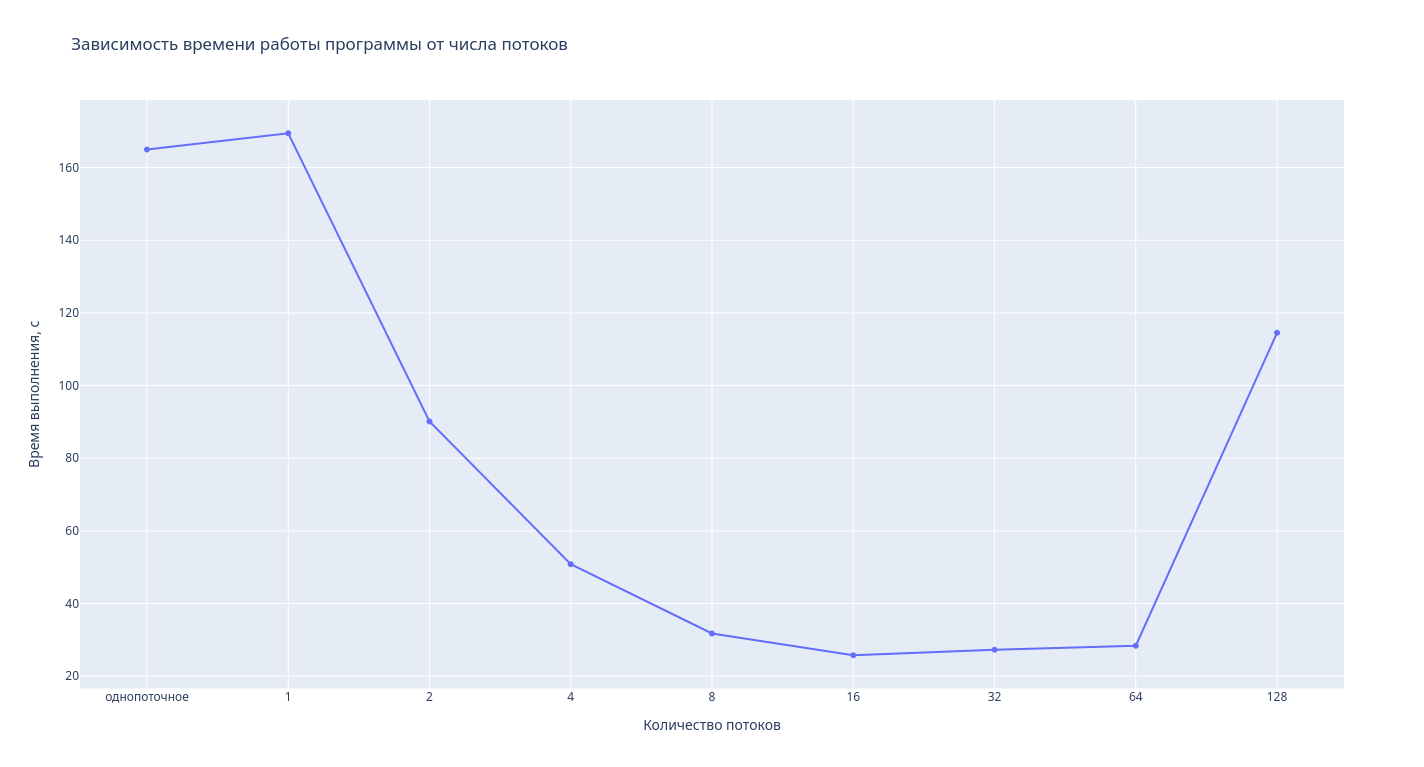
\includegraphics[width=0.9\textwidth]{plot}
	\caption{График временных характеристик разработанных программ}
	\label{plot}
\end{figure}

\begin{longtable}{|r|r|}
	\caption{Временные характеристики разработанных программ (начало)}\label{tbl:time}
	\\
	\hline
	Количество потоков & Время работы, с \\
	\hline
	\endfirsthead
	\caption{Временные характеристики разработанных программ (окончание)}
	\\
	\hline
	Количество потоков & Время работы, с \\
	\hline
	\endhead
	\hline
	\endfoot
	\endlastfoot
	\hline
	\multicolumn{2}{|c|}{Однопоточная реализация} \\
	\hline
	1 & 164.98 \\
	\hline
	\multicolumn{2}{|c|}{Многопоточная реализация} \\
	\hline
	1 & 169.45 \\
	\hline
	2 & 90.11 \\
	\hline
	4 & 50.85 \\
	\hline
	8 & 31.79 \\
	\hline
	16 & 25.78 \\
	\hline
	32 & 27.32 \\
	\hline
	64 & 28.42 \\
	\hline
\end{longtable}

В результате исследования сделан вывод, что использование параллельных вычислений на нативных потоках может ускорить программу, однако использование потоков, больше числа потоков процессора (в случае устройства, на котором проводились замеры >16 потоков), не даст увеличения временной производительности.


\ssr{ЗАКЛЮЧЕНИЕ}

Целью -- разработка ПО, выполняющего скачивание страниц и парсинг рецептов с сайта menunedeli.ru -- была выполнена.

В ходе работы были решены следующие задачи:
\begin{itemize}
	\item рассмотрена структура сайта;
	\item разработано ПО, выполняющее скачивание и парсинг в одном потоке;
	\item разработано многопоточное ПО, выполняющее скачивание и парсинг;
	\item исследованы временные характеристики разработанных программ.
\end{itemize}

В ходе исследования было выявлено, что использование параллельных вычислений на нативных потоках ускоряет программу, однако использование большего числа потоков, чем может выполнять процессор не даёт прироста производительности, а замедляет программу.






